\documentclass[11pt,a4paper]{article}

\usepackage[a4paper,margin=1in]{geometry}
\usepackage{graphicx}
\usepackage{booktabs}
\usepackage{float}
\usepackage{hyperref}
\usepackage{xcolor}
\usepackage{listings}
\usepackage{enumitem}
\usepackage{fancyhdr}

\hypersetup{colorlinks=true,linkcolor=blue,urlcolor=blue}

\pagestyle{fancy}
\setlength{\headheight}{14pt}
\fancyhf{}
\lhead{Computer Networks Laboratory}
\rhead{Assignment 6}
\cfoot{\thepage}

\lstdefinestyle{cstyle}{
  language=C,
  basicstyle=\ttfamily\small,
  numbers=left,
  numberstyle=\tiny,
  frame=single,
  breaklines=true,
  showstringspaces=false,
  keywordstyle=\color{blue},
  commentstyle=\color{gray},
  stringstyle=\color{purple}
}
\lstset{style=cstyle}

\setlength{\parskip}{0.5em}
\setlength{\parindent}{0pt}

\begin{document}

\begin{center}
{\LARGE \textbf{Assignment 6: Error Detection using Checksum and CRC}}\\[4mm]
Simiyon Vinscent Samuel L\\
Register Number: 3122247001062\\
Submission Date: August 18, 2026\\
GitHub Repository: \url{https://github.com/blackscythe123/PCN-assign}
\end{center}

\vspace{2mm}
\hrule
\vspace{4mm}

\section*{Aim}
To build small C programs that show how a receiver can detect transmission errors
without any extra hardware -- first using the 1's complement checksum method locally,
then using a Cyclic Redundancy Check (CRC) sent for real over a TCP socket. The goal is
to actually see a bit error get caught, not just compute a checksum value and call it
done.

\section*{Part (a): Checksum -- End-Around-Carry Addition}
\texttt{checksum.c} does not need sockets, since part (a) of the brief only asks for
sender/receiver logic, not a network transfer -- that requirement is satisfied by part
(b) instead. The program splits the message into 8-bit words (one word per character),
adds them with 1's complement addition, and applies end-around carry: whenever an
addition overflows past 8 bits, the overflow bit is wrapped back around and added into
the sum instead of being discarded. The final checksum is the 1's complement of that
sum.

\begin{lstlisting}[caption={checksum.c -- add\_with\_end\_around\_carry(): the core end-around-carry loop, printing every intermediate sum and carry}]
for (int i = 0; i < count; i++) {
    sum = sum + words[i];
    int carry = 0;

    /* end-around carry: if the addition overflowed past 8 bits,
     * wrap the overflow bit back around and add it to the sum */
    if (sum > 0xFF) {
        sum = (sum & 0xFF) + 1;
        carry = 1;
    }

    printf("  step %2d: word = %3u (0x%02X)  ->  sum = %3u (0x%02X)  carry-out = %d\n",
           i + 1, words[i], words[i], sum & 0xFF, sum & 0xFF, carry);
}
\end{lstlisting}

The receiver side re-adds the data words plus the checksum word using the exact same
function. If nothing was corrupted, that sum comes out as all 1s (255, i.e. 0xFF for an
8-bit word) and the program prints ERROR-FREE. \texttt{main()} runs the whole
sender+receiver simulation twice on the same message ("NETWORKS"): once untouched, and
once with bit 0 of the first transmitted word manually flipped right before the
receiver step, so both outcomes show up side by side in the same run.

For the message "NETWORKS", the sender computed a final sum of 127 (0x7F) and a
checksum of 128 (0x80). In the clean run the receiver's re-sum came to 255 (0xFF) --
all 1s -- and was reported ERROR-FREE. In the corrupted run, flipping bit 0 of the
first word changed it from 78 to 79, and every subsequent intermediate sum in the
receiver's re-addition differed from the clean run; the final sum came to 1 (0x01)
instead of 255, and the program correctly reported ERROR DETECTED.

\begin{figure}[H]
\centering
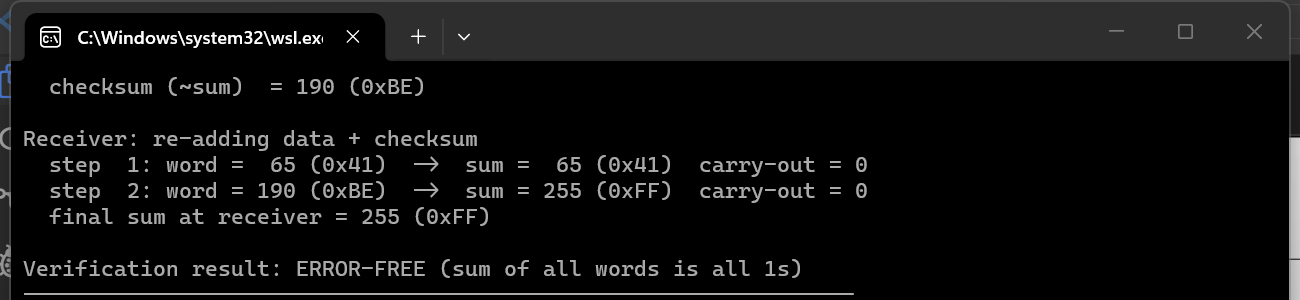
\includegraphics[width=0.85\linewidth]{ss/01_checksum_clean.png}
\caption{checksum.c clean run: intermediate sums/carries for both the sender and
receiver passes, ending in an ERROR-FREE verification.}
\end{figure}

\begin{figure}[H]
\centering
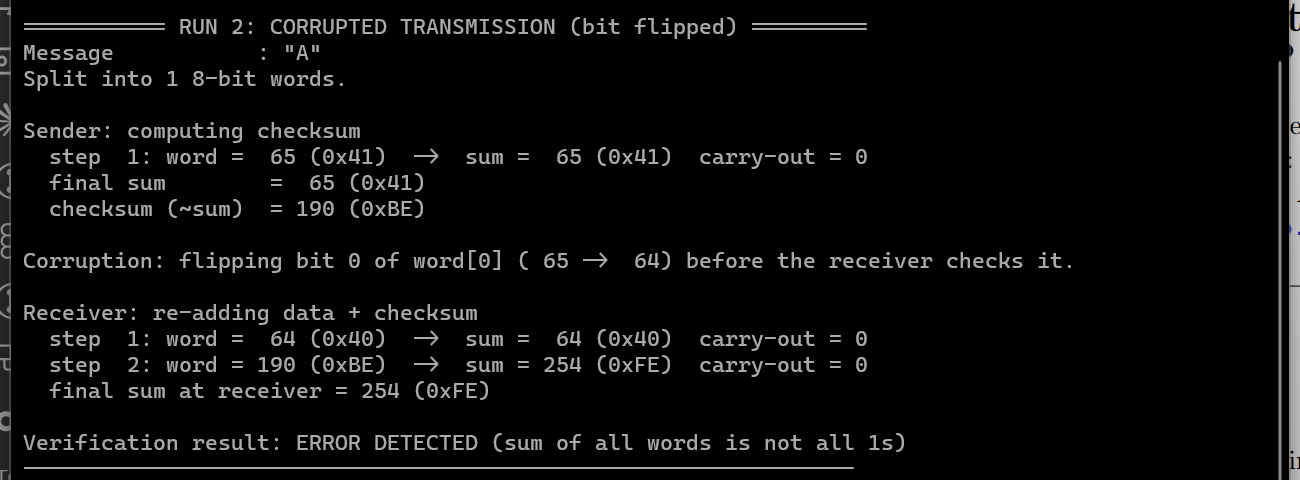
\includegraphics[width=0.85\linewidth]{ss/02_checksum_error.png}
\caption{checksum.c corrupted run: the same message with bit 0 of the first word
flipped before the receiver re-adds it, ending in an ERROR DETECTED verification.}
\end{figure}

\section*{Part (b): CRC over TCP Sockets}
\texttt{crc\_sender.c} and \texttt{crc\_receiver.c} are a real TCP client/server pair
communicating on port 6063. The sender converts the message to its binary equivalent
(8 bits per character), computes the CRC using the generator G(x) = x\^{}4 + x + 1
(bit pattern 10011) via mod-2 polynomial division, and appends the 4 CRC bits to the
data before sending the whole frame over the socket. The receiver divides the entire
received frame (data + CRC) by the same generator; a zero remainder means the frame is
error-free, any non-zero remainder means it was corrupted.

\begin{lstlisting}[caption={crc\_sender.c / crc\_receiver.c -- mod2\_divide(): binary long division by XOR, the core of the CRC computation and verification}]
void mod2_divide(const char *dividend, int dividend_len,
                  const char *generator, int gen_len, char *remainder_out) {
    char temp[256];
    strcpy(temp, dividend);

    for (int i = 0; i <= dividend_len - gen_len; i++) {
        /* only XOR when the leading bit at this position is 1 -
         * that's how binary long division skips over leading zeros */
        if (temp[i] == '1') {
            for (int j = 0; j < gen_len; j++) {
                temp[i + j] = (temp[i + j] == generator[j]) ? '0' : '1';
            }
        }
    }

    int rem_len = gen_len - 1;
    strncpy(remainder_out, temp + (dividend_len - rem_len), rem_len);
    remainder_out[rem_len] = '\0';
}
\end{lstlisting}

To demonstrate an error over the real socket connection, \texttt{crc\_sender} takes an
optional \texttt{corrupt} argument; when passed, it flips one bit inside the already-framed
data (data + CRC) right before sending, and prints exactly which bit changed. The
receiver has no idea whether a given run is clean or corrupted -- it just divides
whatever frame it receives and reports what it finds, which is what makes this a real
test of the detection logic rather than a scripted result.

For the message "HELLO" (binary \texttt{01001000 01000101 01001100 01001100
01001111}), the sender computed a CRC of \texttt{1111}, giving the transmitted frame
\texttt{01001000 01000101 01001100 01001100 01001111 1111}. In the clean run the
receiver divided
that frame by the generator and got a remainder of 0000, reporting the frame
error-free. In the corrupted run, the sender flipped bit position 3 of the frame (0 to
1) before sending; the receiver divided the altered frame and got a non-zero remainder
of 0111, correctly reporting that the frame contained errors.

\begin{figure}[H]
\centering
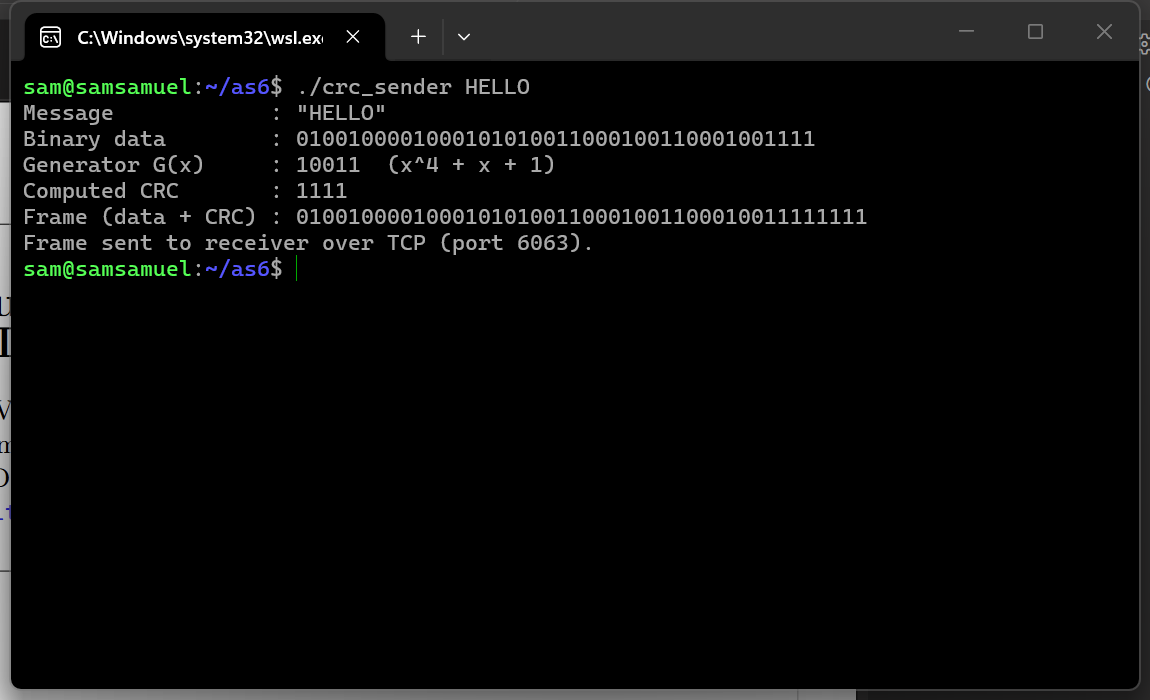
\includegraphics[width=0.85\linewidth]{ss/03_crc_sender.png}
\caption{crc\_sender.c terminal: binary conversion of "HELLO", the generator 10011,
the computed CRC 1111, and the combined frame sent over TCP.}
\end{figure}

\begin{figure}[H]
\centering
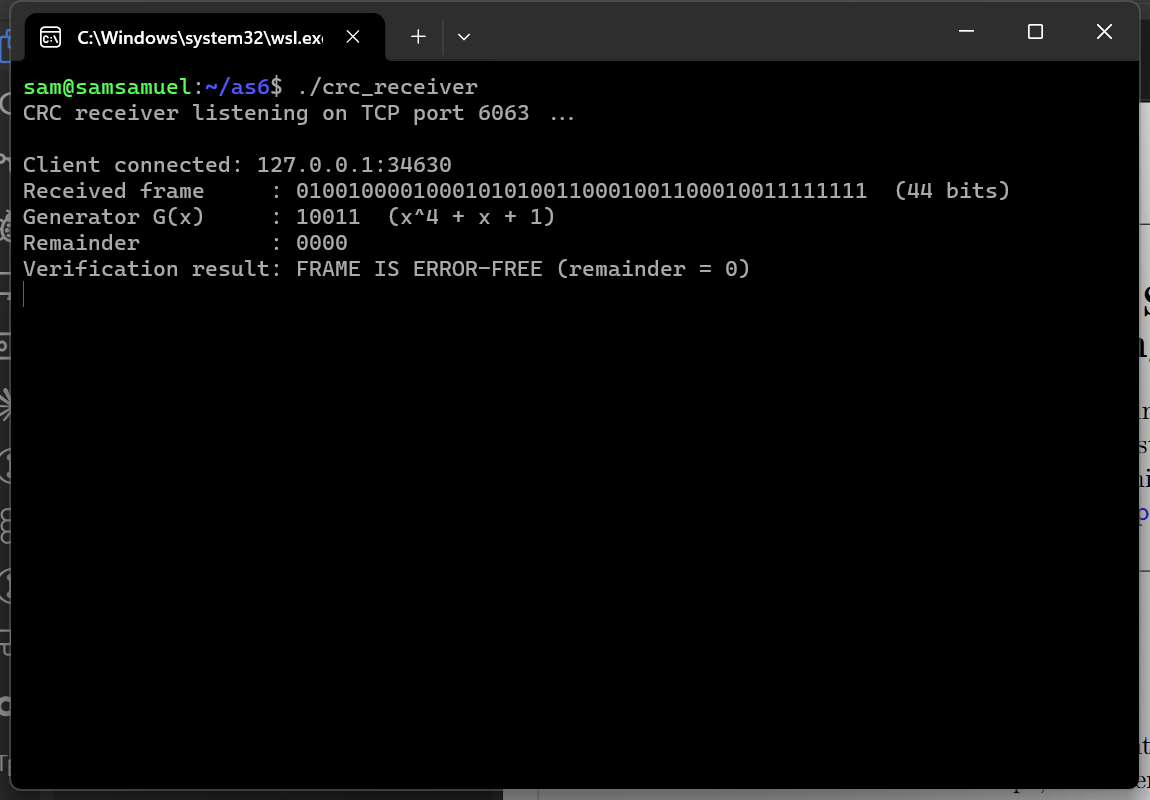
\includegraphics[width=0.85\linewidth]{ss/04_crc_receiver_clean.png}
\caption{crc\_receiver.c terminal for the clean frame: remainder 0000, reported as
error-free.}
\end{figure}

\begin{figure}[H]
\centering
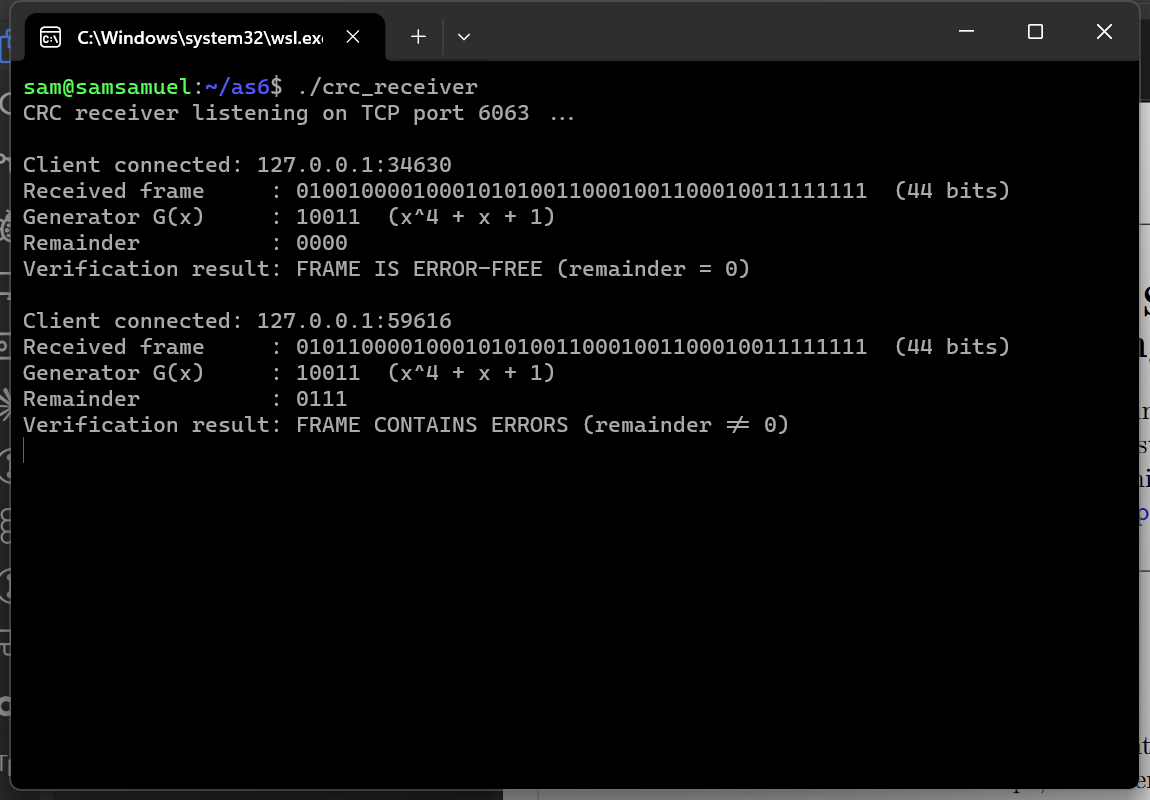
\includegraphics[width=0.85\linewidth]{ss/05_crc_receiver_error.png}
\caption{crc\_receiver.c terminal for the corrupted frame: non-zero remainder 0111,
reported as containing errors.}
\end{figure}

\section*{Learning Outcome}
\begin{itemize}
\item End-around carry is easy to describe but easy to get wrong in code -- the fix is
just "if the sum overflows 8 bits, add the overflow bit back in," but forgetting the
wrap-back step (or wrapping the whole sum instead of just the excess bit) silently
breaks the checksum.
\item CRC division looked intimidating on paper but turned out to just be repeated XOR
at each '1' bit going left to right -- once that clicked, writing \texttt{mod2\_divide}
took a handful of lines, and it is literally the same function on both the sender and
receiver.
\item Running the CRC pair over a real TCP socket (rather than just calling the same
function twice in one program) made it obvious that the receiver genuinely does not
know in advance whether a frame is clean or corrupted -- it only ever sees a remainder,
and everything downstream depends on trusting that remainder is zero.
\end{itemize}

\end{document}
